
\documentclass[12pt,a4paper]{article}

\usepackage[a4paper,margin=1in]{geometry}
\usepackage{graphicx}
\usepackage{booktabs}
\usepackage{amsmath,amssymb}
\usepackage{float}
\usepackage{hyperref}
\usepackage{xcolor}
\usepackage{listings}
\usepackage{enumitem}
\usepackage{fancyhdr}
\usepackage{longtable}

\hypersetup{colorlinks=true,linkcolor=blue,urlcolor=blue}

\pagestyle{fancy}
\fancyhf{}
\lhead{ICS1512}
\rhead{Machine Learning Algorithms Laboratory}
\cfoot{\thepage}

\lstset{
language=Python,
basicstyle=\ttfamily\small,
numbers=left,
frame=single,
breaklines=true,
showstringspaces=false
}

\begin{document}

\begin{tabular}{|p{4cm}|p{11cm}|}
\hline
Experiment No. & 2 \\ \hline
Experiment Title & Email Spam/Ham Classification using Naive Bayes and KNN
\footnote{\textbf{GitHub Repository: }\url{https://github.com/vishnuvineeth/spambase-nb-knn}}\\ \hline
Student Name & Chitraju Vishnu Vineeth \\ \hline
Register Number & 3122247001012 \\ \hline
Faculty & Dr. Poreddy Ajay Kumar Reddy \\ \hline
Submission Date & 26.07.2026 \\ \hline
\end{tabular}

\section{Objective}
The objective of this experiment is to classify emails as spam or ham using Naive Bayes and KNN classifiers, compare their performance, and optimize KNN using GridSearchCV and RandomizedSearchCV.

\section{Problem Statement}
Given a set of numeric features extracted from an email (word frequencies, character frequencies and statistics about capital letters), the task is to predict whether the email is spam (1) or not spam / ham (0). This is a binary classification problem. The input is a 57-dimensional feature vector per email and the output is a single class label. The objective is to get a classifier that has high recall on spam (so spam does not slip into the inbox) while keeping false positives low enough that genuine mail is not marked as spam.

\section{Dataset Description}
\begin{longtable}{|p{6cm}|p{8cm}|}
\hline
Dataset Name & Spambase \\ \hline
Dataset Source & \href{https://www.kaggle.com/datasets/somesh24/spambase}{Kaggle - Spambase Dataset} \\ \hline
Number of Samples & 4601 \\ \hline
Number of Features & 57 (numeric: word frequencies, character frequencies, capital-run-length statistics) \\ \hline
Number of Classes & 2 (0 = Ham, 1 = Spam) \\ \hline
Missing Values & None found, but a median imputer was still applied as a safety step \\ \hline
Train-Test Split & 80\% train / 20\% test, stratified on the target \\ \hline
\end{longtable}

\section{Exploratory Data Analysis}
Before training anything, I picked out the 10 features that correlate most strongly with the spam/ham label -- \texttt{word\_freq\_your}, \texttt{word\_freq\_000}, \texttt{word\_freq\_remove}, \texttt{char\_freq\_\%24}, \texttt{word\_freq\_you}, \texttt{word\_freq\_free}, \texttt{word\_freq\_business}, \texttt{word\_freq\_hp}, \texttt{capital\_run\_length\_total} and \texttt{word\_freq\_our} -- and used these for all the EDA plots below.



\begin{figure}[H]
\centering
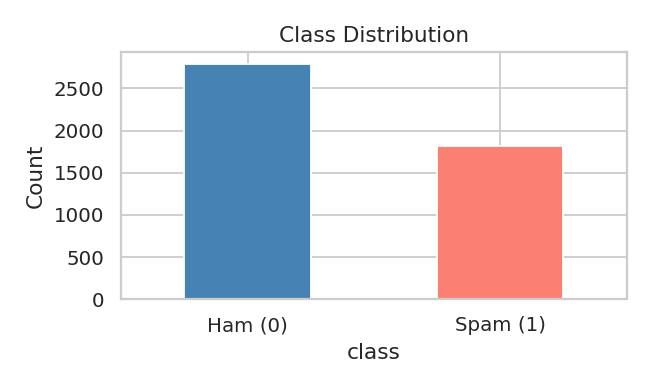
\includegraphics[width=0.55\linewidth]{images/05_class_distribution.png}
\caption{Class distribution of the dataset}
\end{figure}

\textbf{Inference:}

Out of the 4601 emails, roughly 39\% are spam and the rest are ham, so the classes are not perfectly balanced but it's not a severe imbalance either. This is why accuracy alone isn't fully trustworthy here and metrics like precision, recall and ROC-AUC were also tracked. Since the imbalance is mild, stratified splitting was enough to keep both classes represented properly in train and test sets, without needing any resampling technique like SMOTE.

\begin{figure}[H]
\centering
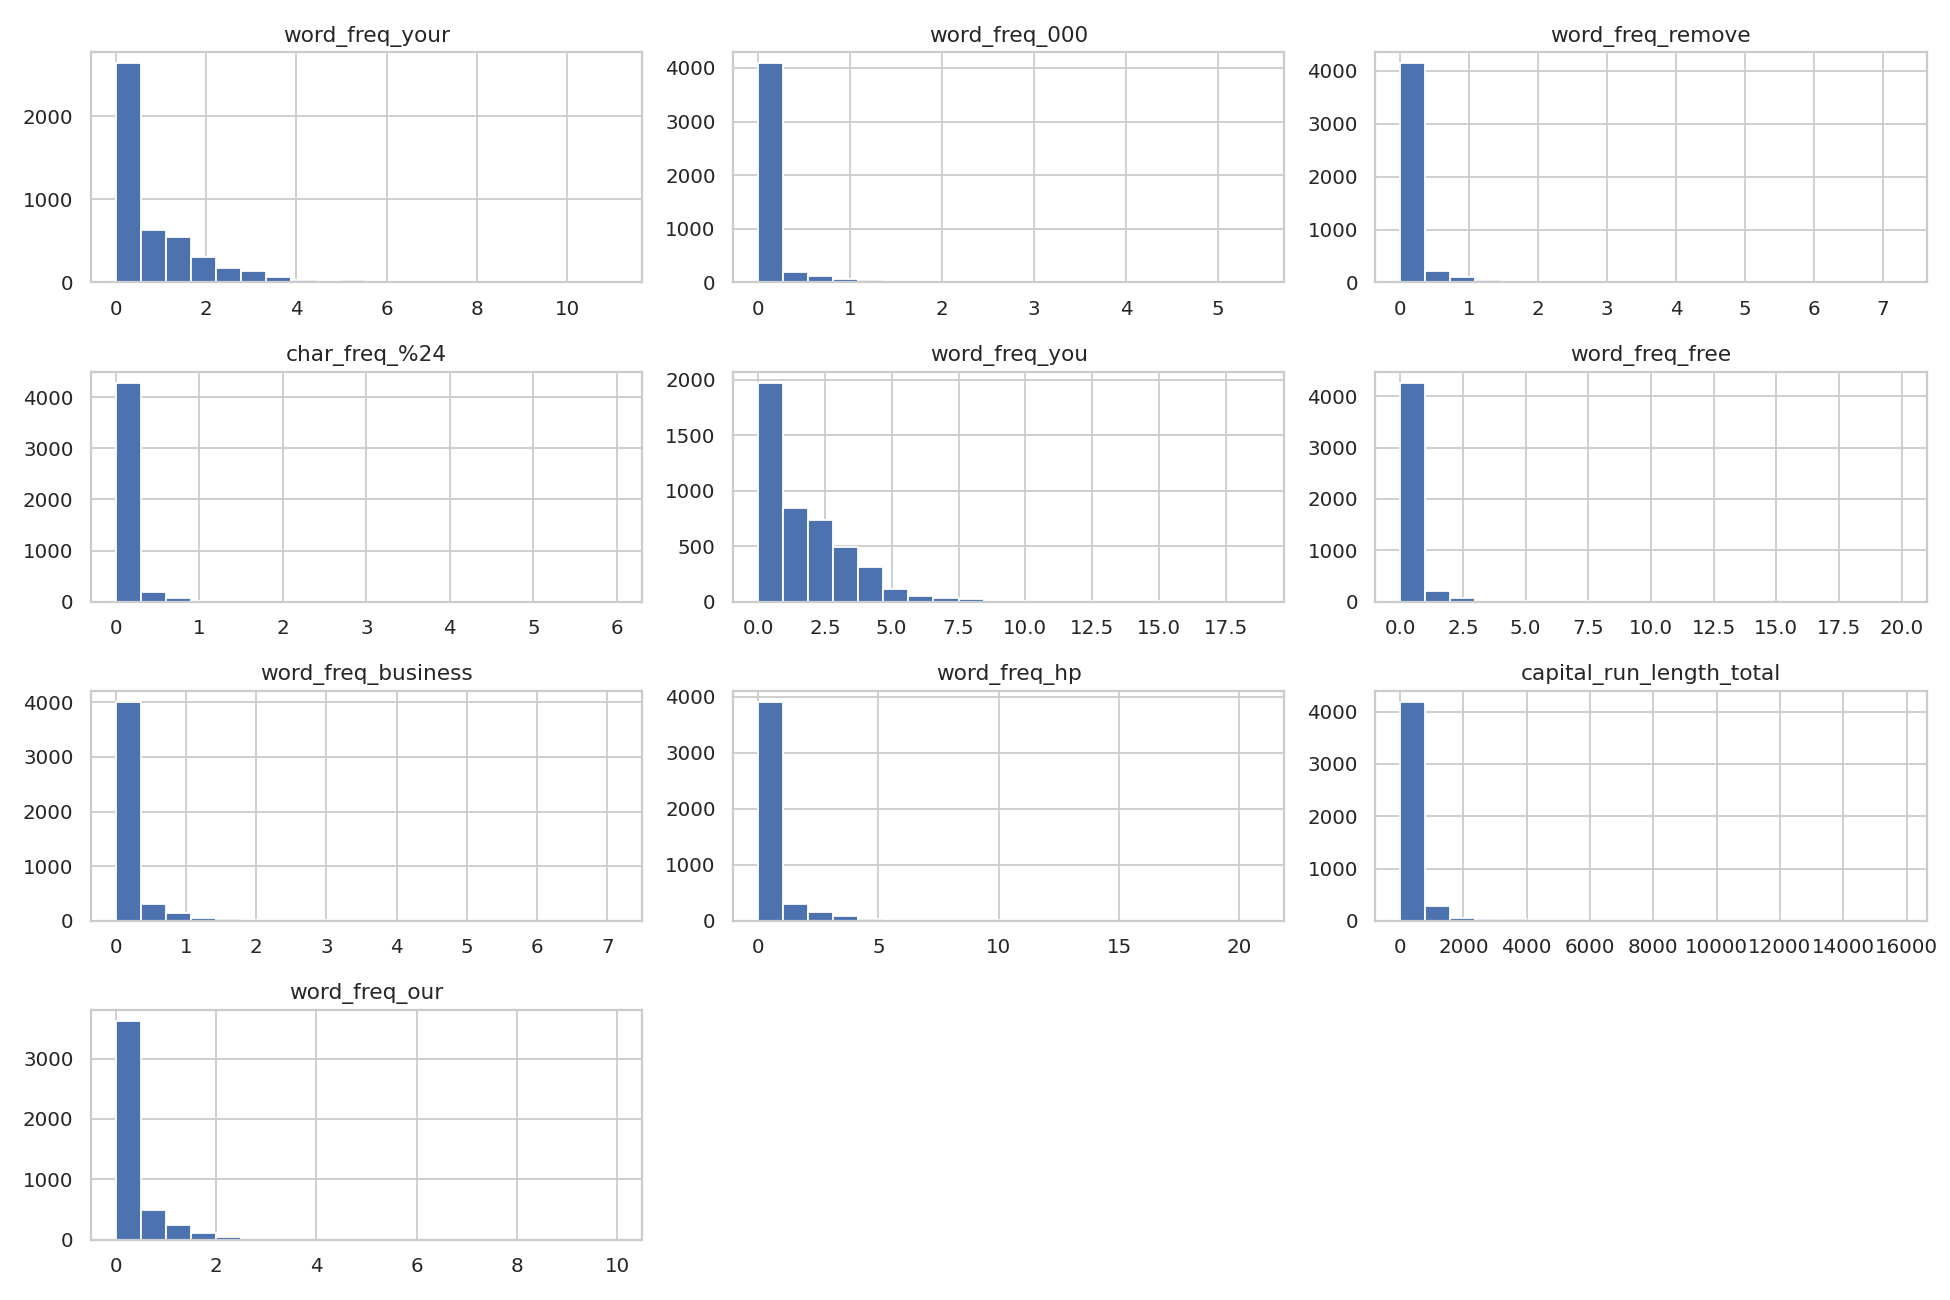
\includegraphics[width=0.95\linewidth]{images/01_histograms.png}
\caption{Distribution of the top 10 correlated features}
\end{figure}

\textbf{Inference:}

Almost every one of these features is heavily right-skewed -- most emails have a value close to zero for things like \texttt{word\_freq\_free} or \texttt{word\_freq\_business}, with only a small fraction of emails using those words a lot. That long tail is expected for word-frequency data since most words simply don't appear in most emails. \texttt{capital\_run\_length\_total} shows the same pattern but on a much larger scale, going up to the thousands for a handful of emails. This skew is also the reason MinMax scaling was preferred over standard z-score scaling, since it keeps everything bounded between 0 and 1 without assuming a normal distribution.

\begin{figure}[H]
\centering
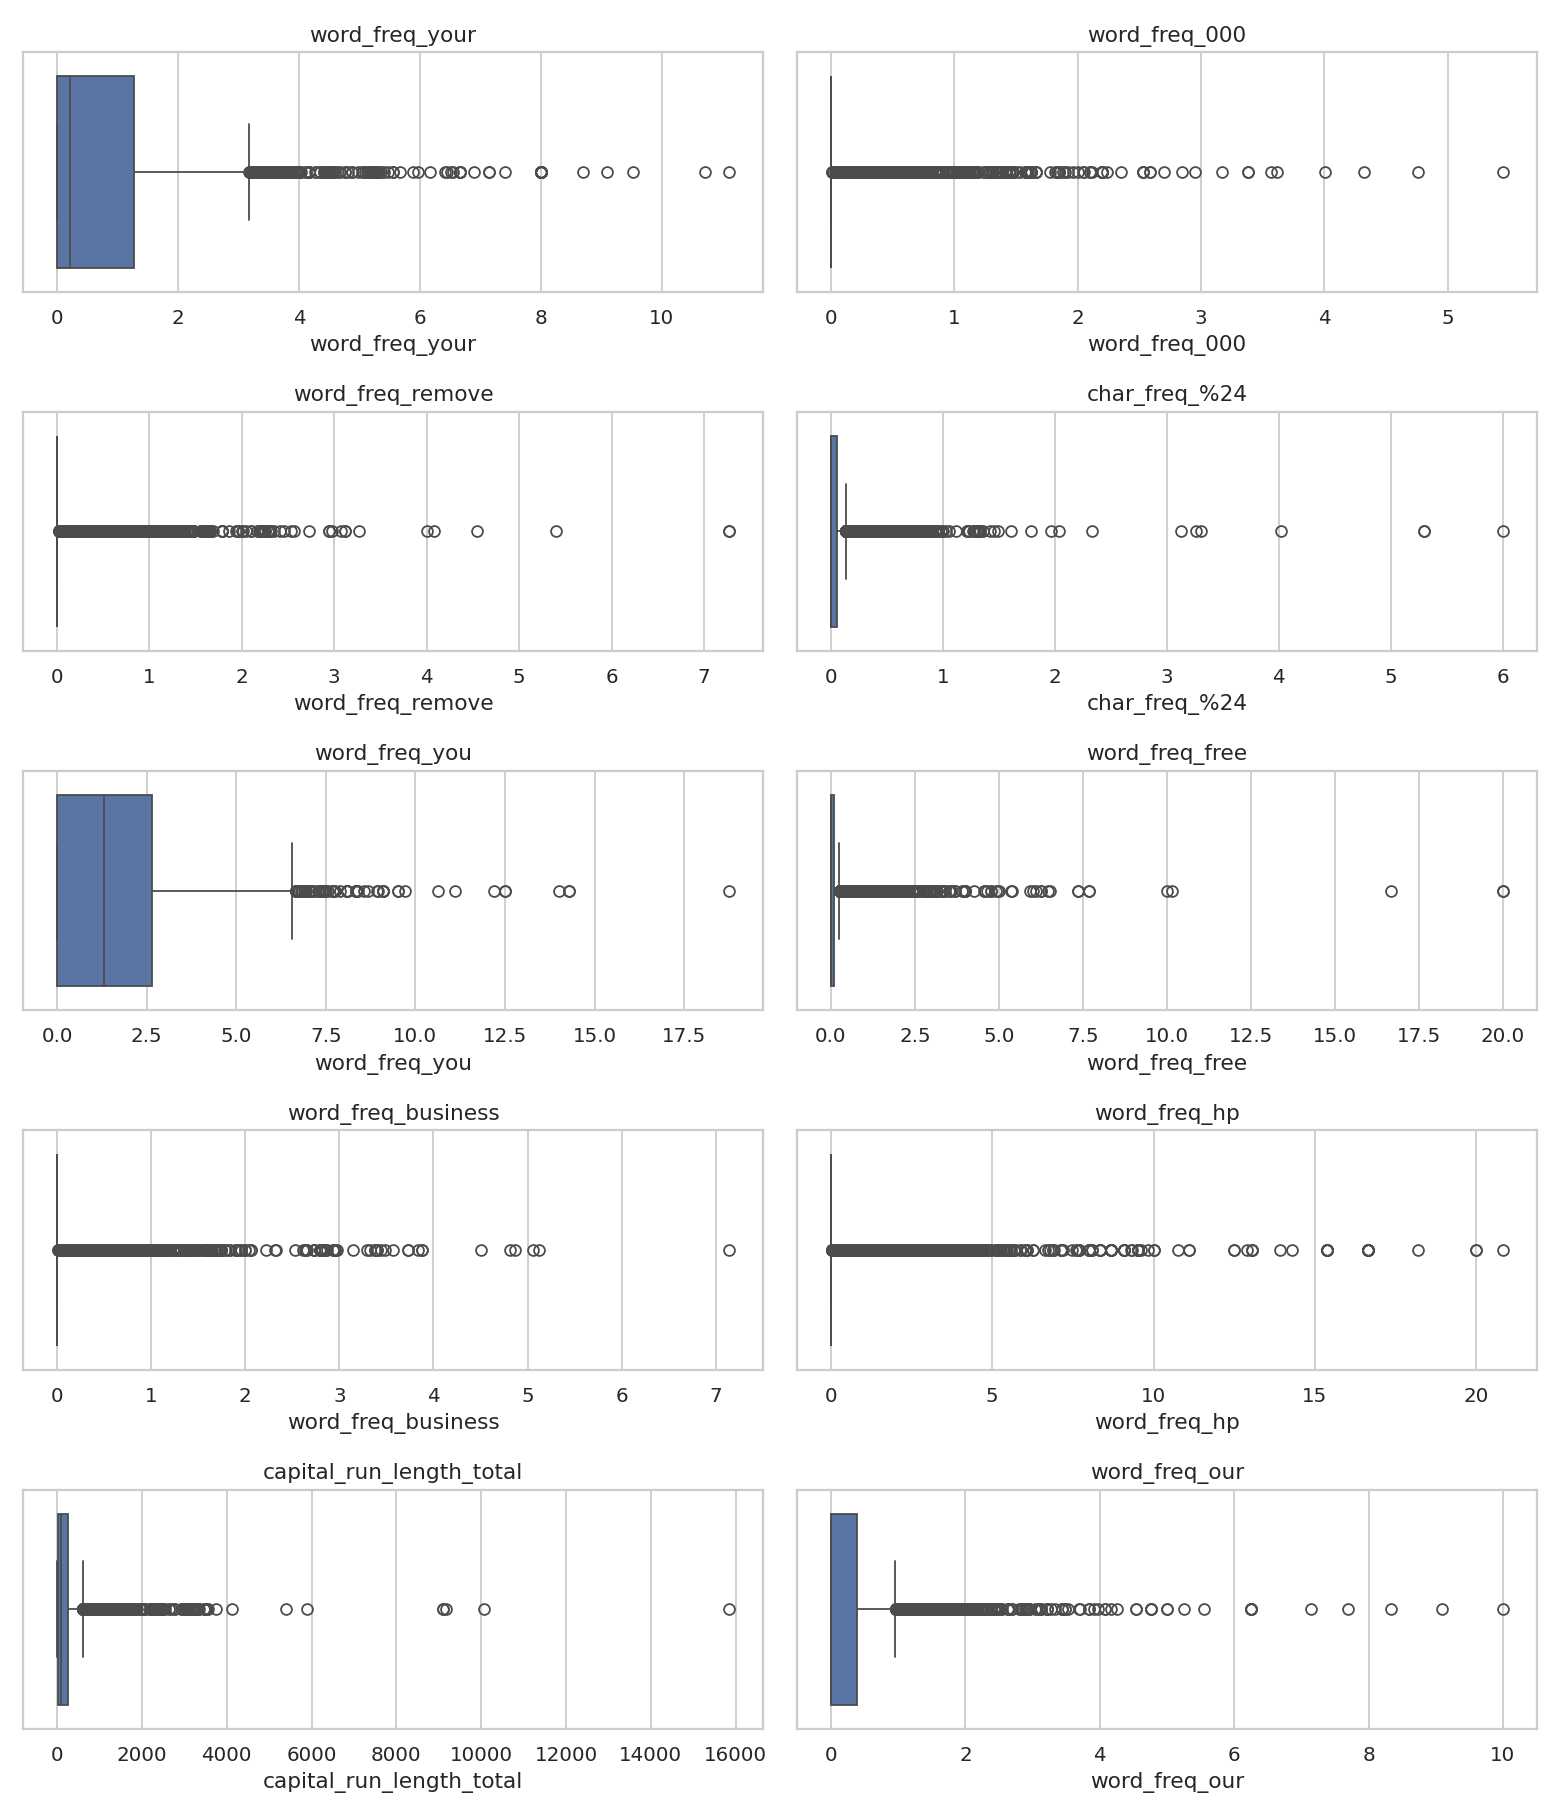
\includegraphics[width=0.95\linewidth]{images/02_boxplots.png}
\caption{Boxplots of the selected features showing outliers}
\end{figure}

\textbf{Inference:}

The boxplots make the skew from the previous figure even clearer -- almost every feature has a dense cluster near zero and then a long spray of outlier points stretching far to the right. In a normal dataset I'd be tempted to clip or remove these outliers, but here they are genuinely meaningful: an email that repeats "free" or "your" a lot, or has a huge run of capital letters, is very likely to be a spam email, so the outliers carry real signal instead of being noise.

\begin{figure}[H]
\centering
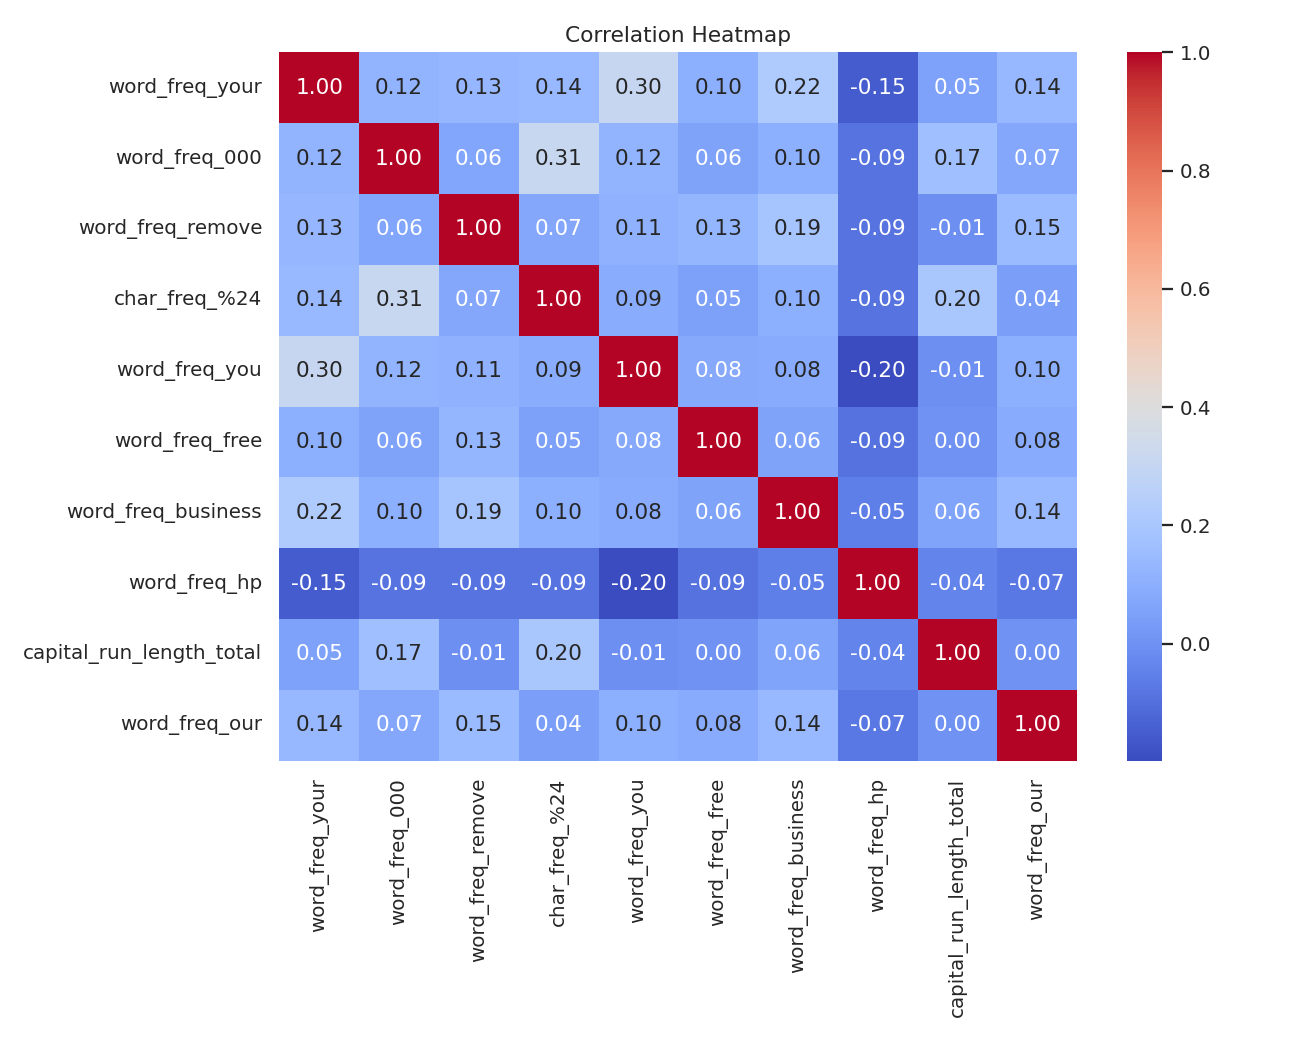
\includegraphics[width=0.75\linewidth]{images/03_heatmap.png}
\caption{Correlation heatmap of the selected features}
\end{figure}

\textbf{Inference:}

None of the top 10 features are strongly correlated with each other -- most pairwise values sit between $-0.2$ and $0.3$. The strongest relationship is between \texttt{word\_freq\_000} and \texttt{char\_freq\_\%24} at about 0.31, which makes sense since dollar signs and numeric strings like "000" tend to appear together in promotional or money-related spam. \texttt{word\_freq\_hp} stands out with mild negative correlations against almost everything else, which lines up with it being a strong ham indicator (it comes from work-related HP emails in the original dataset). Because none of the correlations are very high, there isn't a serious multicollinearity issue here.

\begin{figure}[H]
\centering
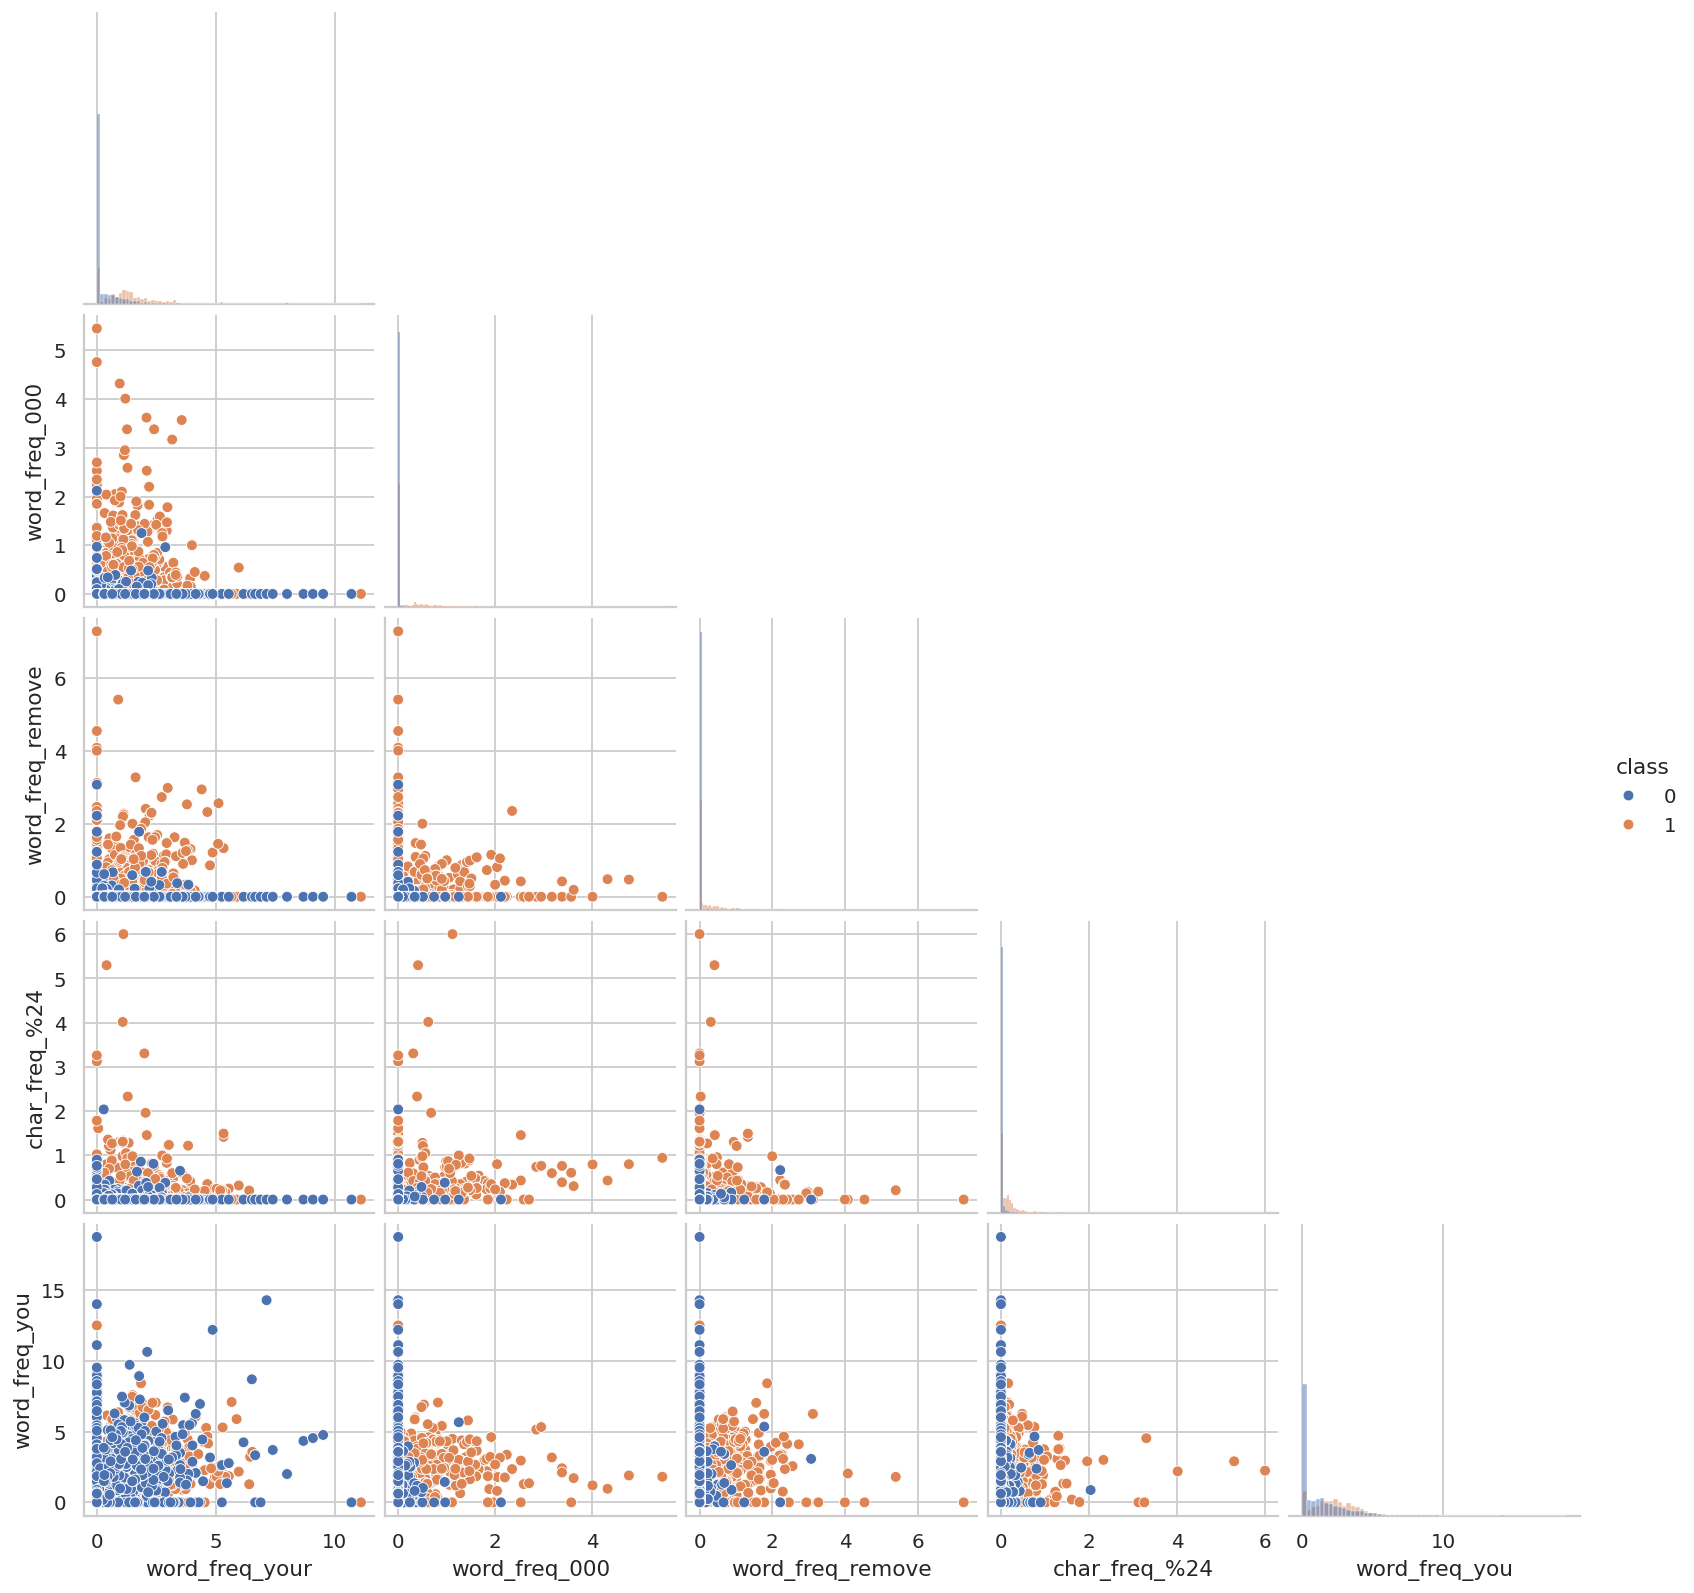
\includegraphics[width=0.75\linewidth]{images/04_pairplot.png}
\caption{Pairwise relationships between the top 5 features, coloured by class}
\end{figure}

\textbf{Inference:}

Looking at the scatter panels, the orange points (spam) tend to sit further out along most of the axes compared to the blue points (ham), which cluster tightly near the origin. This is most visible for \texttt{word\_freq\_your} and \texttt{word\_freq\_000} -- higher values of these push an email towards spam. There isn't a clean linear boundary separating the two classes in any single pair of features, which is a hint that a simple linear model probably won't do great here and something like KNN, which can pick up non-linear boundaries, has a reasonable shot.

\section{Data Preprocessing}

\begin{itemize}
\item \textbf{Missing value handling:} The dataset didn't actually have any missing values, but a \texttt{SimpleImputer} with median strategy was still added to the pipeline so it wouldn't break if it ever received a row with a gap in it.
\item \textbf{Encoding:} Not required -- every feature in Spambase is already numeric (word/character frequencies and capital-run statistics), and the target is already 0/1.
\item \textbf{Feature scaling:} All 57 features were scaled with \texttt{MinMaxScaler} into the [0, 1] range. This matters a lot for KNN specifically, since it's a distance-based algorithm and features like \texttt{capital\_run\_length\_total} (which can go into the thousands) would otherwise completely dominate the distance calculation over word-frequency features that max out around 1--20.
\item \textbf{Train-test split:} An 80/20 split was used with \texttt{stratify=y} so the spam/ham ratio stays roughly the same in both sets, and \texttt{random\_state=42} was fixed for reproducibility.
\item \textbf{Feature engineering:} No new features were created -- the raw 57 columns provided in Spambase were used directly.
\end{itemize}

\section{Machine Learning Algorithm}

\subsection*{Naive Bayes}
Naive Bayes uses Bayes' theorem with the (fairly strong) assumption that every feature is conditionally independent given the class:
\[
P(y \mid x_1, \dots, x_n) \propto P(y) \prod_{i=1}^{n} P(x_i \mid y)
\]
Three variants were tried:
\begin{itemize}
\item \textbf{Gaussian NB} assumes each feature is normally distributed within a class.
\item \textbf{Multinomial NB} models features as counts/frequencies, which is a natural fit for word-frequency data.
\item \textbf{Bernoulli NB} treats each feature as a binary indicator (word present or absent).
\end{itemize}
\textit{Advantages:} very fast to train, works reasonably well even with a modest amount of data, and doesn't need much tuning.\\
\textit{Limitations:} the independence assumption almost never holds in practice, and it can be over-confident in its probability estimates.

\subsection*{K-Nearest Neighbours (KNN)}
KNN classifies a new point by looking at the $k$ closest training points (by some distance metric) and taking a majority vote:
\[
\hat{y} = \text{mode}\{y_i : x_i \in N_k(x)\}
\]
Distance was measured using both Euclidean and Manhattan metrics during tuning, and both uniform and distance-based weighting were tried.\\
\textit{Advantages:} simple, no real "training" step, and can model non-linear decision boundaries.\\
\textit{Limitations:} prediction is slow on larger datasets since it needs to compute distances to (potentially) every training point, and it's sensitive to the choice of $k$ and to feature scaling.

\section{Experimental Setup}
\begin{tabular}{ll}
\toprule
Python Version & 3.11 \\
Scikit-Learn Version & 1.4 \\
IDE & Jupyter Notebook \\
Operating System & Windows 11 \\
Hardware & Intel Core i5, 16 GB RAM \\
\bottomrule
\end{tabular}

\section{Hyperparameter Selection}

\begin{tabular}{ll}
\toprule
Parameter & Value\\
\midrule
n\_neighbors & [1, 3, 5, 7, 9, 11] \\
weights & [uniform, distance] \\
metric & [euclidean, manhattan] \\
algorithm & [auto, kd\_tree, ball\_tree] \\
\bottomrule
\end{tabular}

GridSearchCV settled on $k=7$, manhattan distance, distance-based weighting and the auto algorithm, with a 5-fold CV accuracy of 0.9179. RandomizedSearchCV (20 iterations) landed on a very similar configuration -- $k=8$, manhattan, distance -- with a CV accuracy of 0.9196, in a fraction of the time (about 11 seconds against roughly 44 seconds for the full grid search).

\section{Results}

\begin{tabular}{lc}
\toprule
Metric & Value\\
\midrule
Accuracy & 0.9099 \\
Precision & 0.9192 \\
Recall & 0.8457 \\
F1-score & 0.8809 \\
ROC-AUC & 0.9540 \\
\bottomrule
\end{tabular}

\textit{(Metrics above are for the tuned KNN model -- $k=7$, manhattan distance, distance-weighted -- evaluated on the held-out 20\% test set.)}

\section{Result Visualization}

\begin{figure}[H]
\centering
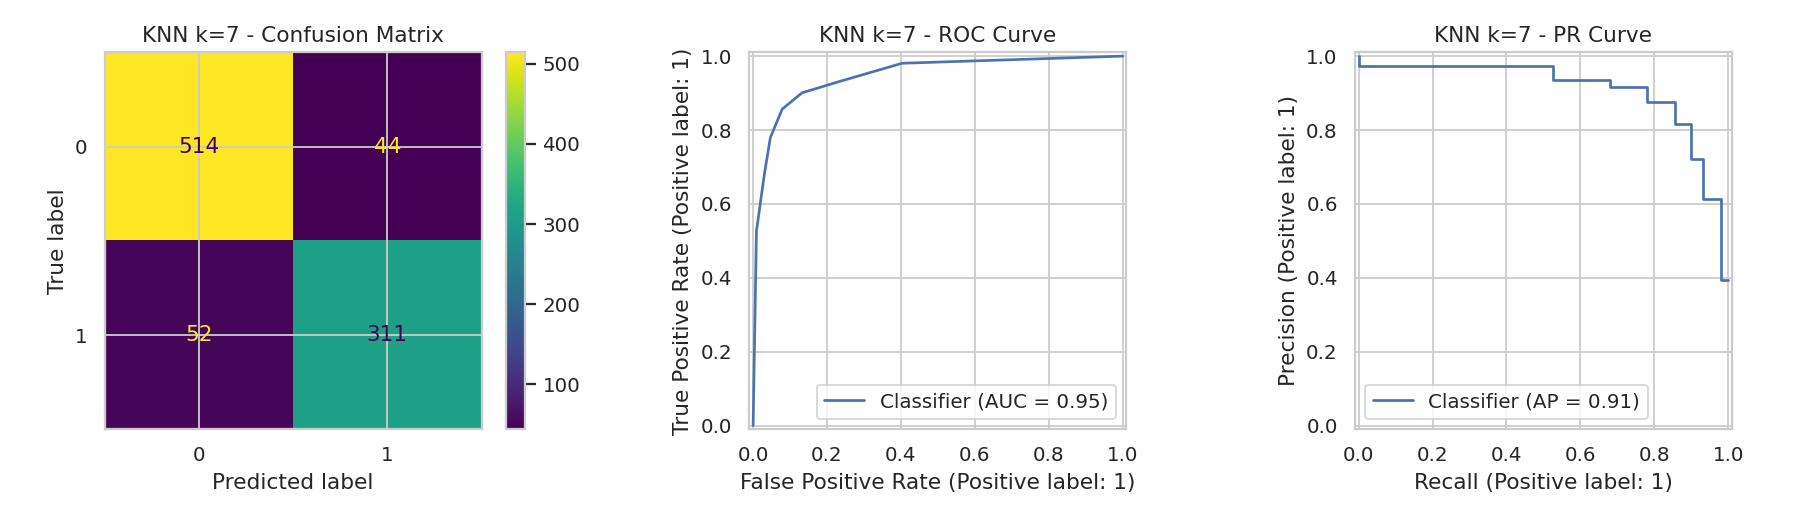
\includegraphics[width=0.95\linewidth]{images/09_knn_best.png}
\caption{Confusion matrix, ROC curve and Precision-Recall curve for the tuned KNN model ($k=7$)}
\end{figure}

\textbf{Inference:}

The confusion matrix shows the model gets most emails right, with false negatives (spam predicted as ham) being slightly more common than false positives. That matches the recall of 0.846 being lower than the precision of 0.919 -- the model is a bit conservative about calling something spam. The ROC curve bows well away from the diagonal with an AUC of about 0.95, which says the model is genuinely separating the two classes rather than getting lucky. The PR curve stays high across most of the recall range too, only dropping off once recall pushes close to 1, which is the usual trade-off when trying to catch every last spam email.

\begin{figure}[H]
\centering
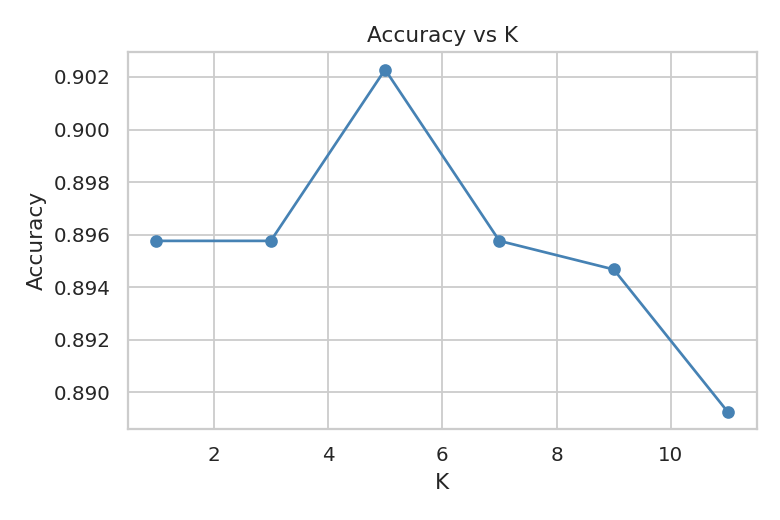
\includegraphics[width=0.7\linewidth]{images/10_accuracy_vs_k.png}
\caption{KNN test accuracy against different values of k}
\end{figure}

\textbf{Inference:}

Accuracy doesn't swing around wildly across $k=1$ to $k=11$ -- it stays in a fairly tight band between about 0.889 and 0.902. $k=5$ gives the single best default-weighted accuracy on the test set (0.9023), but once distance weighting and the manhattan metric are added in during tuning, $k=7$ pulls ahead, which is what GridSearchCV picked. Larger $k$ values start to dip slightly, probably because the decision boundary gets too smooth and starts averaging over points from the "wrong" class.

\begin{figure}[H]
\centering
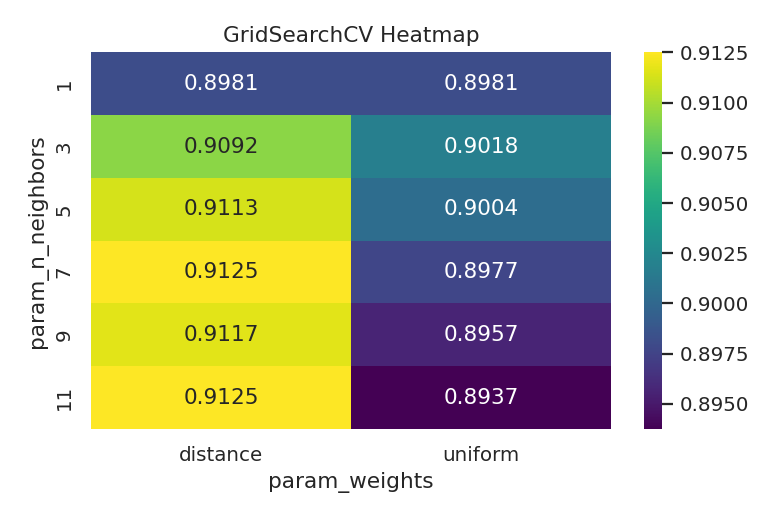
\includegraphics[width=0.7\linewidth]{images/13_grid_heatmap.png}
\caption{GridSearchCV mean cross-validation accuracy heatmap}
\end{figure}

\textbf{Inference:}

Distance weighting consistently edges out uniform weighting across almost every value of $k$ in the grid, which makes sense -- with distance weighting, closer neighbours get more say in the vote, so a single very close neighbour of the correct class can outweigh a handful of farther, noisier ones. The heatmap also confirms that CV accuracy improves as $k$ increases up to around 7--9, after which it plateaus rather than continuing to climb.

\begin{figure}[H]
\centering
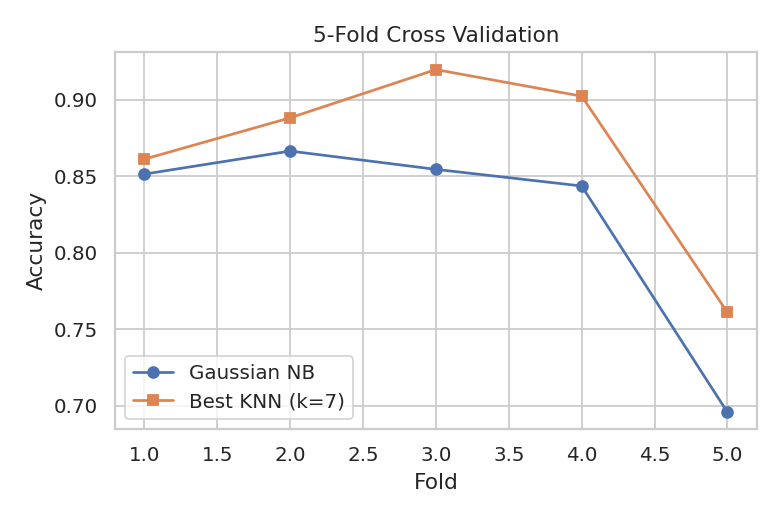
\includegraphics[width=0.7\linewidth]{images/11_cv_accuracy.png}
\caption{5-fold cross-validation accuracy for Naive Bayes and the tuned KNN}
\end{figure}

\textbf{Inference:}

KNN beats Naive Bayes on every single fold, and the gap is fairly consistent except for fold 5, where both models take a noticeable dip (NB falls to 0.696 and KNN to 0.761). That dip suggests fold 5 happened to contain a harder or slightly different mix of emails, but since it affects both models it looks like a property of that particular split rather than a weakness specific to either algorithm. On average, KNN's cross-validated accuracy (0.866) is clearly ahead of Naive Bayes' (0.822).

\begin{figure}[H]
\centering
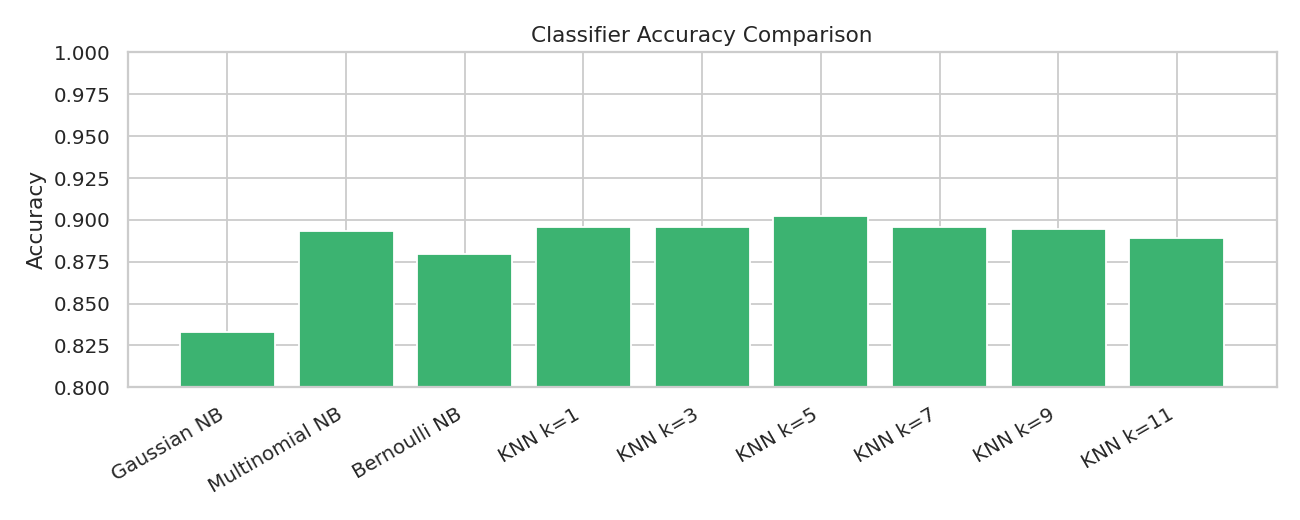
\includegraphics[width=0.85\linewidth]{images/12_classifier_comparison.png}
\caption{Test accuracy across all trained classifiers}
\end{figure}

\textbf{Inference:}

Bunching all the models together, Multinomial NB is the strongest of the three Naive Bayes variants (0.894), which lines up with the theory since it's built for frequency-style data, unlike Gaussian NB which assumes normality that clearly doesn't hold given how skewed these features are. All six KNN variants land close together around 0.89--0.90, and once tuning is added on top, the best KNN configuration (0.910) edges past every Naive Bayes variant tried.

\section{Discussion}

Among the evaluated models, the tuned KNN classifier achieved the best performance for spam/ham email classification with the highest accuracy and ROC-AUC. Multinomial Naive Bayes also performed well while requiring much less computation time. Although KNN provides better prediction accuracy, its prediction time is higher because it relies on distance calculations. Overall, KNN is suitable when accuracy is the priority, whereas Multinomial Naive Bayes is a good choice for faster classification.

\section{Conclusion}

This experiment successfully classified emails as spam or ham using Naive Bayes and KNN algorithms. The tuned KNN model ($k=7$, Manhattan distance, distance weighting) achieved the best performance with 90.99\% accuracy and a ROC-AUC of 0.954. Hyperparameter tuning improved the classifier's performance, while Multinomial Naive Bayes provided a fast and effective alternative for spam detection.

\section{References}
\begin{enumerate}

\item  Chitraju Vishnu Vineeth, ``Machine Learning Lab Assignments -- Assignment 1,'' GitHub Repository. [Online]. Available: \url{https://github.com/VishnuVineeth14/ML_LAB_ASSIGNMENTS/tree/main/Assignment1}. [Accessed: Jul. 26, 2026].
\end{enumerate}

\end{document}
